\section{TiKZ in mathcha}
\tikzset{every picture/.style={line width=0.75pt}} %set default line width to 0.75pt        

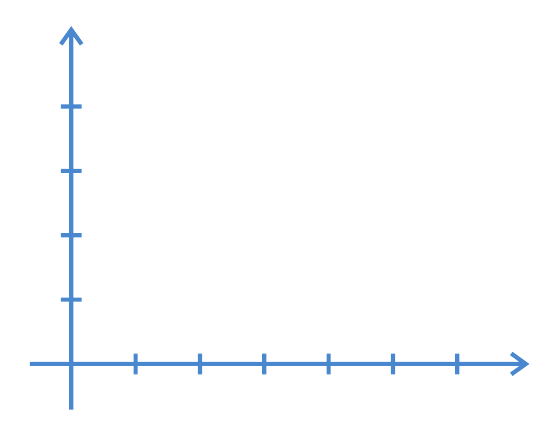
\begin{tikzpicture}[x=0.75pt,y=0.75pt,yscale=-1,xscale=1]
%uncomment if require: \path (0,235); %set diagram left start at 0, and has height of 235

%Shape: Axis 2D [id:dp048941842347560494] 
\draw [color={rgb, 255:red, 73; green, 135; blue, 206 }  ,draw opacity=1 ][line width=1.5]  (41,177) -- (280,177)(61,16) -- (61,199) (273,172) -- (280,177) -- (273,182) (56,23) -- (61,16) -- (66,23) (92,172) -- (92,182)(123,172) -- (123,182)(154,172) -- (154,182)(185,172) -- (185,182)(216,172) -- (216,182)(247,172) -- (247,182)(56,146) -- (66,146)(56,115) -- (66,115)(56,84) -- (66,84)(56,53) -- (66,53) ;
\draw   ;




\end{tikzpicture}